\usetikzlibrary{arrows,shapes,positioning}
\usetikzlibrary{calc,decorations.markings}

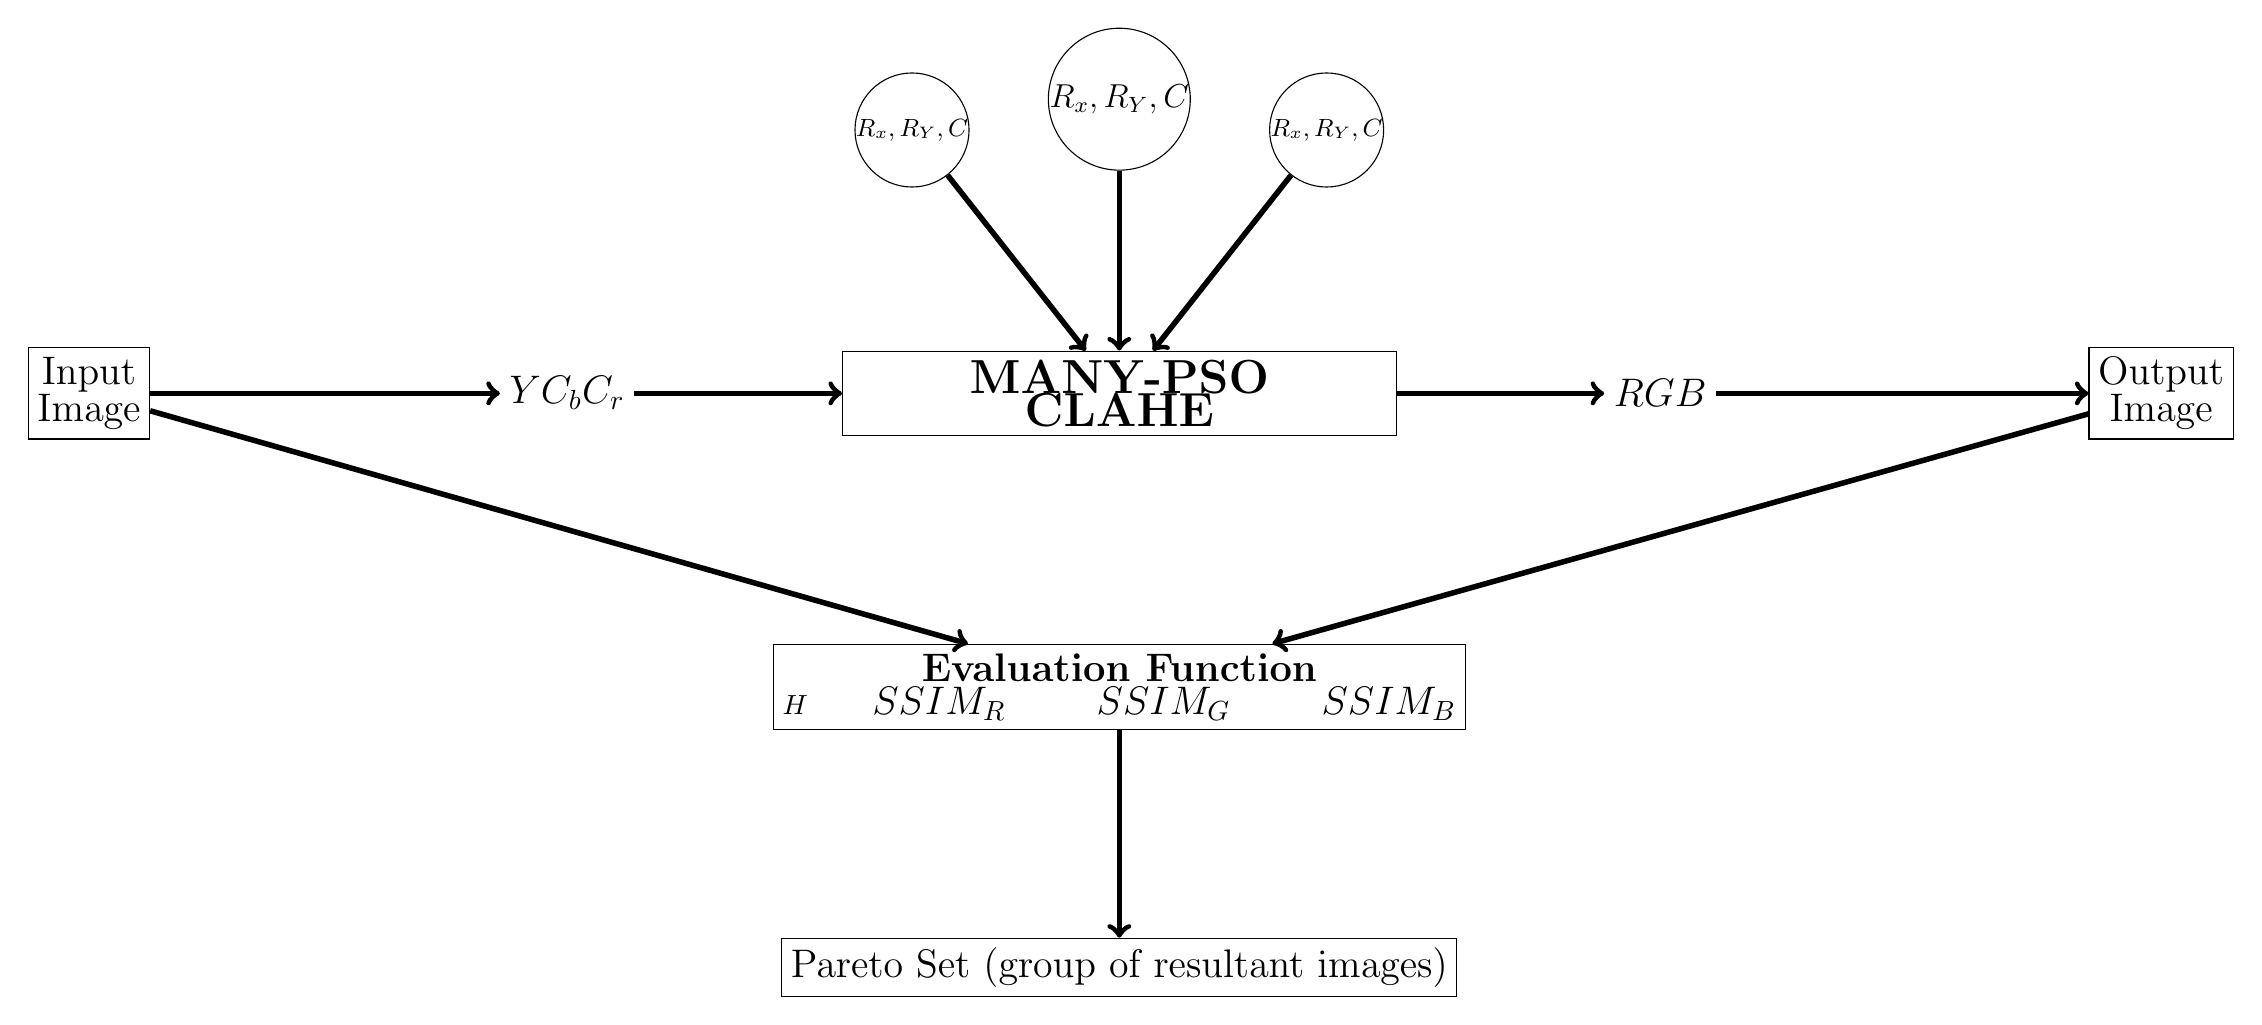
\begin{tikzpicture}

%textos

%\node[draw,align=center] at (3,4) {\textbf{MANY-PSO-CLAHE}};
                                   
\node[draw,align=center,minimum width=200pt] (manypsoclahe) {\LARGE \textbf{MANY-PSO} \\ \LARGE \textbf{CLAHE}};

\node[draw,align=center,below= 75pt of manypsoclahe] (evaluationfunctions) {\Large \textbf{Evaluation Function}\\ $\mathscr{H}$ \qquad \Large $SSIM_R$ \qquad $SSIM_G$ \qquad $SSIM_B$};
                                   
\node[draw,align=center,below= 75pt of evaluationfunctions] (paretoset) {\Large Pareto Set (group of resultant images)};

\node[draw,align=center,left= 250pt of manypsoclahe] (inputimage) {\Large Input \\ \Large Image};

\node[draw,align=center,right= 250pt of manypsoclahe] (outputimage) {\Large Output \\ \Large Image};

\node[draw,circle,minimum size=1cm,inner sep=0pt,above left= 65pt and -40pt of manypsoclahe] (partic1) {\small $\mathscr{R}_x,\mathscr{R}_Y,\mathscr{C}$};

\node[draw,circle,minimum size=1cm,inner sep=0pt,above = 65pt of manypsoclahe] (partic2) {\large $\mathscr{R}_x,\mathscr{R}_Y,\mathscr{C}$};

\node[draw,circle,minimum size=1cm,inner sep=0pt,above right= 65pt and -40pt of manypsoclahe] (partic3) {\small $\mathscr{R}_x,\mathscr{R}_Y,\mathscr{C}$};

\node[align=center,left= 75pt of manypsoclahe] (ycrcb) {\Large $YC_bC_r$};

\node[align=center,right= 75pt of manypsoclahe] (rgb) {\Large $RGB$};

\draw[->,draw=black,solid,line width=2pt, to path={-- (\tikztotarget)}]
  (partic1) edge (manypsoclahe) (partic2) edge (manypsoclahe)
  (partic3) edge (manypsoclahe)
  (inputimage) edge (ycrcb)
  (ycrcb) edge (manypsoclahe)
  (manypsoclahe) edge (rgb)
  (rgb) edge (outputimage)
  (outputimage) edge (evaluationfunctions)
  (inputimage) edge (evaluationfunctions)
  (evaluationfunctions) edge (paretoset);

\end{tikzpicture}